\section{Configuration}
\label{04_configuration}

\subsection{Fixed Frequency Value}
\label{subsec:04_fixedFrequencyVal}

In order to decide on a fixed frequency for the phase method,
resulting errors of different frequency were evaluated.
For this, all measurements in \cref{subsec:04_labMeasurements}
of the robot 26 at the center point are utilized.
As the \ac{RMSE} in \cref{fig:04_diffFc} shows, for frequencies larger
than 2024,1\si{\hertz} the errors increase minimally with growing frequency.
With a frequency of 2024,1\si{\hertz}, error is largest.
Therefore, the fixed frequency is set to 2411,7\si{\hertz}.
% -------------------------------------------------------------
\begin{figure}[ht]
	\centering
		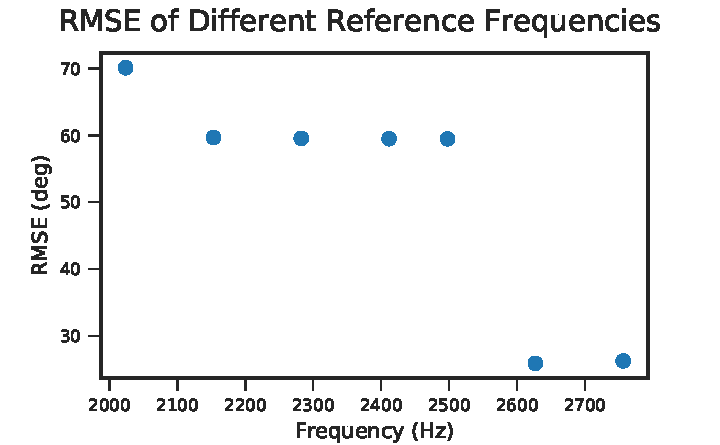
\includegraphics[]{figures/evaluation/phase_fc_rmse}
	\caption{Result of all measurements for Nao 26 to compare different
	fixed frequency values.}
	\label{fig:04_diffFc}
\end{figure}
% -------------------------------------------------------------